%%%%%%%%%%%%%%%%%%%%%%%%%%%%%%%%%%%%%%%%%%%%%%%%%%%%%%%%%%%%%%%%%%
\section{Red de comunicación \glsentryshort{6g}}
\label{sec:6g}

Las redes de comunicación de sexta generación, están en desarrollo para ofrecer una conectividad aún más rápida, confiable y eficiente que las generaciones anteriores. A medida que la demanda de datos continúa creciendo exponencialmente y surgen nuevas aplicaciones y tecnologías, como el \gls{iot}, la realidad aumentada y la \gls{ai}, se espera que el \gls{6g} proporcione una infraestructura de red sólida y escalable para satisfacer estas necesidades futuras. Los principales puntos claves de esta nueva generación se pueden resumir en los siguientes puntos.

\begin{itemize}

    \item Velocidad y capacidad extremadamente altas: Una de las principales características del \gls{6g} será la velocidad y capacidad extremadamente altas, superando con creces las capacidades del \gls{5g}. Se espera que el \gls{6g} alcance velocidades de terabits por segundo, lo que permitirá una transmisión de datos ultra rápida y un soporte eficiente para aplicaciones de alta demanda, como son la transmisión de video en 8K, realidad virtual y realidad aumentada de alta calidad.

    \item Latencia ultrabaja: El \gls{6g} aspira a lograr una latencia ultrabaja, reduciendo aún más el tiempo de respuesta de la red. Se espera que la latencia en el \gls{6g} sea de solo unos pocos milisegundos, lo que permitirá aplicaciones en tiempo real de misión crítica, como cirugías remotas, vehículos autónomos y aplicaciones de realidad virtual y aumentada altamente interactivas.

    \item Conectividad ubicua: El \gls{6g} tiene como objetivo proporcionar conectividad ubicua, extendiéndose más allá de las áreas urbanas y llegando a áreas remotas y rurales haciendo uso de radio enlaces satelitales de orbita baja (LEO). Se espera que el \gls{6g} aborde la brecha digital y brinde conectividad global a nivel mundial, permitiendo una mayor inclusión digital y oportunidades equitativas para todos.

    \item Integración de tecnologías emergentes: El \gls{6g} se construirá sobre tecnologías emergentes, como inteligencia artificial (IA), \gls{ml}, llegando a proponer la computación cuántica y nanotecnología. Estas tecnologías avanzadas permitirán el desarrollo de sistemas de red más inteligentes y autónomos, optimizando la eficiencia y la capacidad de adaptación de la red.

    \item Sostenibilidad y eficiencia energética: El \gls{6g} se enfocará en la sostenibilidad y la eficiencia energética para reducir su impacto ambiental. Se espera que las redes \gls{6g} sean más eficientes en términos de consumo de energía, al tiempo que brinden una mayor capacidad y rendimiento. Además, se explorarán nuevas técnicas de transmisión de energía y comunicación inalámbrica para impulsar la eficiencia energética en dispositivos y redes.

\end{itemize}

\subsection{Tecnologías habilitadoras}

Como se comentó en el capítulo de introducción (Capitulo \ref{ch:intro}), esta nueva generación aún es prematura y no tiene unos estándares claros y definidos sobre como se va a llevar a cabo, sin embargo, ya empieza a haber propuestas sobre las tecnologías habilitadoras que harán del \gls{6g} una realidad tarde o temprano. Desde el proyecto líder europeo  6G-Flagship y la organiazción One6G ya se apuntan a una serie de tecnologías claves, las cuales, se indican a continuación.

\subsubsection{Banda de los THz}

Según se ha indicado, con el \gls{6g}, se espera que fusione los mundos digital y físico en todas sus dimensiones, brindando a los usuarios una experiencia holográfica, háptica y multisensorial. Según la \gls{itu}, estas aplicaciones surgirán en la próxima década y se caracterizarán por requerir comunicaciones altamente exigentes \cite{fg20192030}. Además, algunas aplicaciones demandarán funcionalidades que los sistemas móviles actuales no proporcionan, como una detección precisa, mapeo y localización. Un ejemplo destacado de caso de uso es la telepresencia holográfica\footnote{\url{https://blogthinkbig.com/peoplefirst/telepresencia-holografica}}. La transmisión de hologramas 3D en su forma más básica requiere una capacidad de más de 4 Tbps \cite{giordani2020toward}. La capacidad de detectar y comprender el entorno permitirá a la red predecir el movimiento de los usuarios sin información explícita, creando así una experiencia inmersiva a distancia. Asimismo, las comunicaciones de alta velocidad de datos y baja latencia necesarias para la automatización de fábricas se beneficiarán de las transmisiones a terabits por segundo (Tbps). \\
\\
Con el fin de satisfacer esta necesidad, las comunicaciones en terahercios (THz) se han identificado como una opción prometedora para la capa física en 6G, ya que tienen el potencial de permitir velocidades de datos de terabits por segundo y ofrecer servicios de detección, mapeo y localización \cite{latva2020key}. En la Conferencia Mundial de Radiocomunicaciones de 2019 (CMR2019)\footnote{\url{https://www.itu.int/es/ITU-R/conferences/wrc/2019}}, la \gls{itu} identificó un espectro de 137 GHz entre 275 y 450 GHz que se puede utilizar para las comunicaciones en terahercios \cite{kurner2020impact}. Esto se suma al espectro ya asignado por debajo de los 275 GHz, lo que proporciona un total de 160 GHz en la gama de sub-terahercios. En 2017, el grupo de trabajo IEEE 802 completó el primer estándar inalámbrico para frecuencias portadoras alrededor de los 300 GHz (IEEE Std 802.15.3d-2017) \cite{ieee2017ieee, petrov2020ieee}. Esto establece una base sólida para el desarrollo y la implementación de las comunicaciones en terahercios en el contexto de 6G. Aunque, también aparecen nuevos retos de capa física a solventar, dado que según subimos en frecuencia la atenuación de la señal aumentará de forma cuasi-proporcional.

\subsubsection{Próxima generación de \glsentryshort{mimo}}

Utilizar múltiples antenas conlleva una serie de ventajas fundamentales. Estas ventajas están condicionadas por el conocimiento del canal en el transmisor y/o receptor, las propiedades del canal de propagación (como características multitrayecto y atenuación) y el tipo de enlace, ya sea punto a punto o multiusuario. Además, la cooperación entre las señales transmitidas o recibidas y el procesamiento conjunto de las antenas también juegan un papel importante.\\
\\
El diseño de soluciones de múltiples entradas y múltiples salidas (\gls{mimo}, por sus siglas en inglés) depende en gran medida del escenario específico que se considere, pero generalmente se suele plantear una descomposición generica del canal donde se vaya a trabajar en una serie de subcanales $M$ paralelos (Ver figura \ref{fig:fig_3}). No existe una única solución \gls{mimo} universal. Al diseñar sistemas \gls{mimo}, es esencial tener en cuenta las limitaciones prácticas y encontrar un equilibrio entre las ganancias básicas del \gls{mimo} \cite{ordonez2011fundamental}. Las ganancias de estos sistemas se pueden resumir en los siguientes puntos.

\begin{itemize}
    \item Ganancia por procesado en \textit{Array}. La combinación coherente de $M$ antenas, sin importar la distancia entre ellas o si funcionan en modo de transmisión o recepción, puede mejorar la relación señal-ruido (SNR) en un máximo de 10 veces. En otras palabras, la SNR puede mejorarse en un máximo de $10*log_{10}(M)\:dB$ mediante la técnica de combinación de las $M$ antenas. Esto se logra mediante la formación de haz (\textit{beamforming}), la cual nos permite ``apuntar" de una forma más precisa con el lóbulo principal de nuestro diagrama de radiación al sistema receptor. Existen múltiples técnicas para llevar a cabo un \textit{beamforming}, desde alimentaciones diferentes en las $M$ antenas, a desfases, jugando con la combinación resultante de todas ellas.

    \item Multiplexación y ganancia por acceso múltiple. La combinación de antenas proporciona otra ventaja fundamental, la capacidad de eliminar señales no deseadas controlando los pesos de las antenas de tal manera que los frentes de onda superpuestos se cancelen en canales específicos. Esto se aprovecha de varias formas, como en el caso del acceso múltiple por división espacial (SDMA) en canales multiusuario o en la multiplexación espacial en canales punto a punto. En general, se asume que el número de señales es igual o menor al número de antenas. Con un conjunto de $M$ antenas, es posible separar hasta $M$ usuarios sin interferencias. Esta capacidad de separación espacial permite mejorar significativamente la eficiencia y el rendimiento de los sistemas de comunicación, al permitir la transmisión simultánea y la recepción de múltiples señales independientes en el mismo espectro.

    \item   La diversidad de antenas y \textit{hardening} del canal. Son conceptos relacionados con los desvanecimientos causados por la propagación multitrayecto. A pequeña escala, estos desvanecimientos espaciales pueden ocurrir debido a la presencia de múltiples trayectos de señal. Si las distancias entre las antenas son lo suficientemente grandes, cada antena experimentará un canal que no está correlacionado con las demás antenas. Este fenómeno se aprovecha transmitiendo o recibiendo información redundante en paralelo a través de las múltiples antenas. Al hacerlo, se logra una diversidad espacial en el sistema, lo que implica que cada antena experimenta diferentes condiciones de desvanecimiento. Como resultado, si una antena se ve afectada por un desvanecimiento, es probable que otras antenas no se vean afectadas de la misma manera. Esta diversidad de antenas proporciona robustez al canal frente a los desvanecimientos. Al transmitir o recibir información redundante a través de múltiples antenas, se pueden mitigar los efectos de los desvanecimientos selectivos de trayecto y mejorar la calidad de la señal.
\end{itemize}

\begin{figure}[h!]
    \centering
    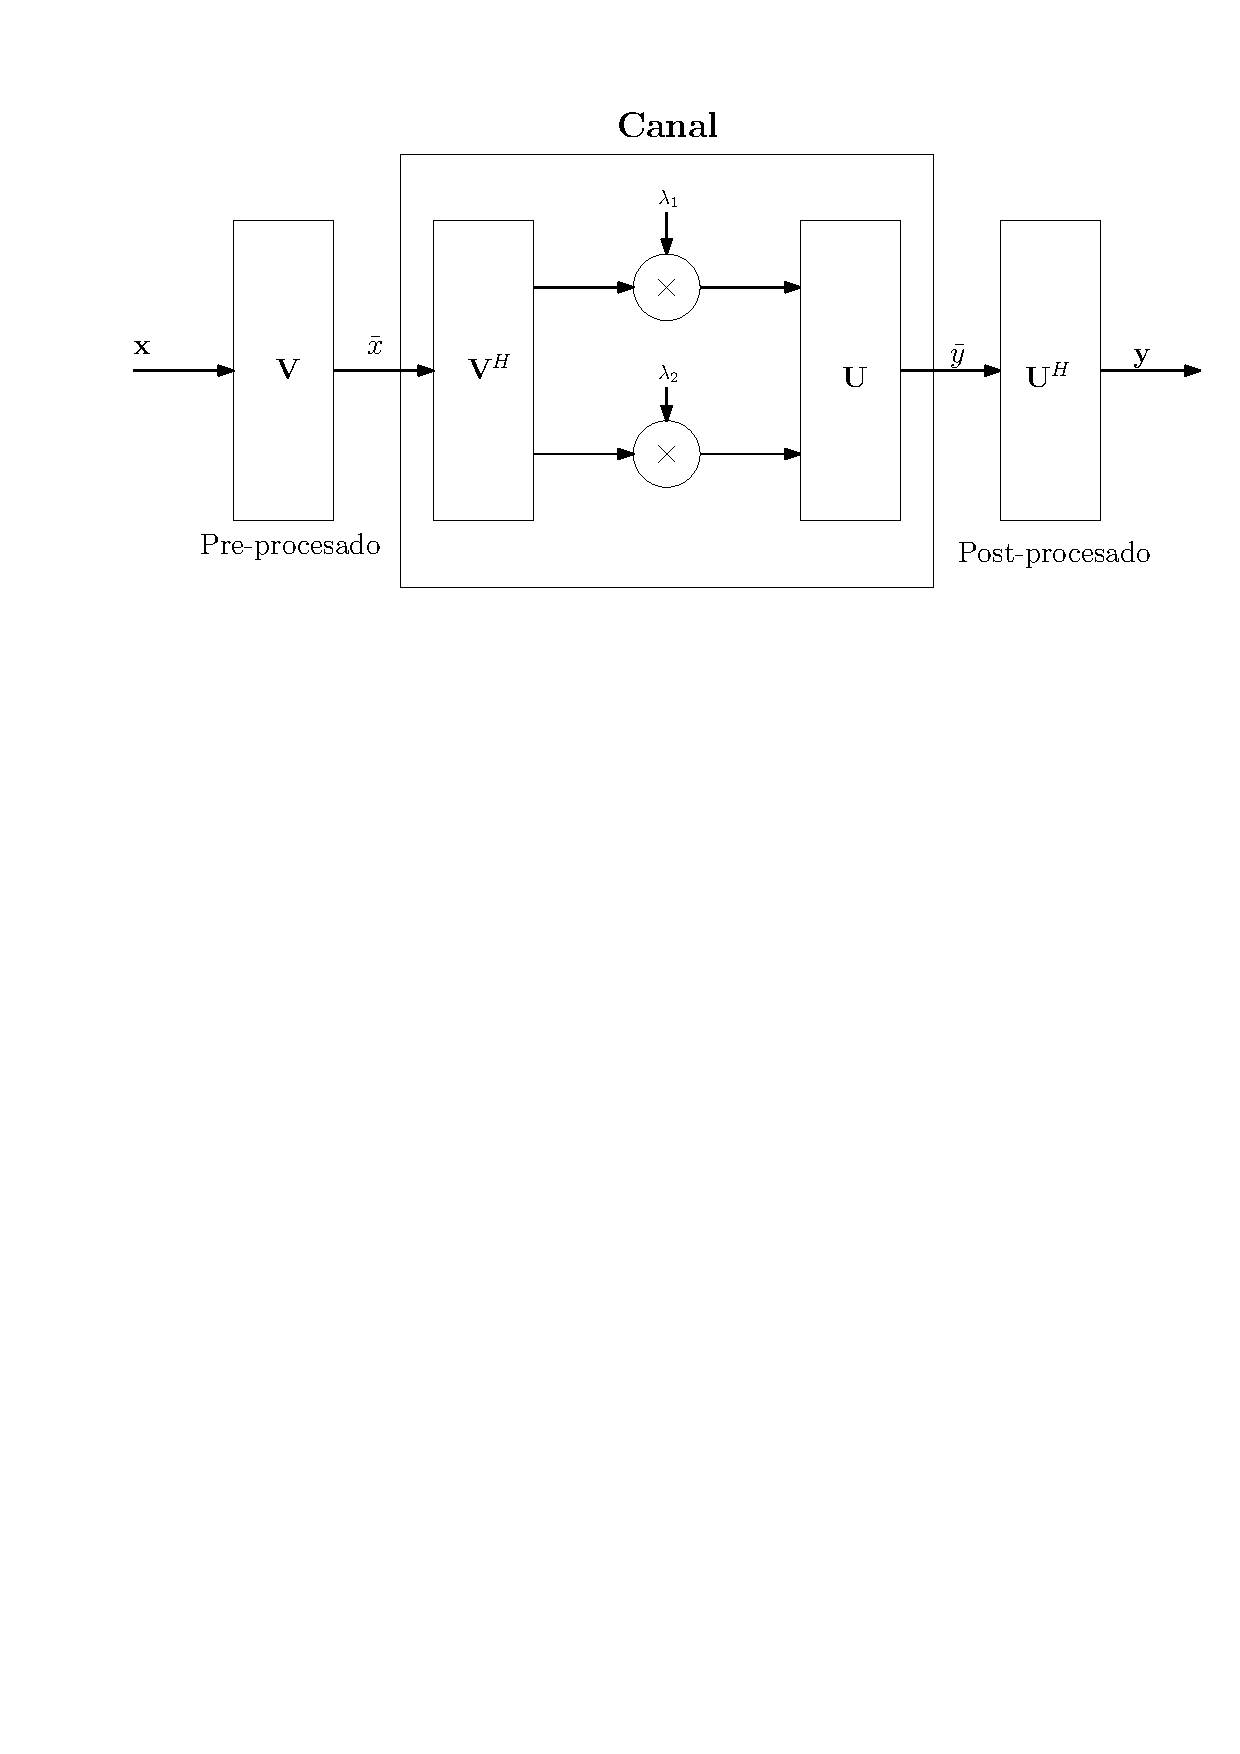
\includegraphics[width=0.8\textwidth]{archivos/img/teoria/fig_3.pdf}
    \caption{Descomposición genérica de un canal \gls{mimo} en subcanales paralelos}
    \label{fig:fig_3}
\end{figure}

Con el fin de aprovechar al máximo las ganancias del \gls{mimo}, se ha observado una tendencia hacia arrays de antenas cada vez más grandes, ya sea en configuraciones coubicadas, conocido como ``massive MIMO" \cite{bjornson2016massive}, o distribuidos en toda la zona de servicio. En respuesta a esta tendencia, se introdujo el \gls{mimo} de dimensión completa en la versión 13 del estándar LTE. En el caso de 5G NR, el 3GPP especificó 32 antenas en la versión 15, y se espera que este número aumente en futuras versiones para habilitar el \gls{mimo} masivo. En el ámbito de la \gls{6g}, se ha introducido el concepto de múltiples matrices D-MIMO, conocido como \gls{mimo} masivo modular (mmMIMO) \cite{jeon2021mimo}. Este concepto incluye D-MIMO estructurado y diversas variantes de CoMP (Coordinated Multi-Point), incluyendo la transmisión conjunta como casos especiales. En \cite{jeon2021mimo} se presentan ejemplos de implementación de prototipos y se describen los pasos de normalización asociados.\\
\\
Estas tendencias en la evolución del \gls{mimo} reflejan la importancia de utilizar arrays de antenas cada vez más grandes y distribuidos para mejorar el rendimiento y la capacidad de los sistemas de comunicación. El enfoque en el \gls{mimo} masivo y el mmMIMO en el \gls{6g} tiene como objetivo proporcionar una mayor capacidad y eficiencia espectral, así como mejorar la cobertura y la calidad de la señal en entornos complejos.

\subsubsection{\glsentryshort{ai} federada y distribuida}

La \gls{ai} y el \gls{ml} se encuentran entre las tecnologías fundamentales que están moldeando el futuro de Internet tal cual lo conocemos. Estas tecnologías están revolucionando la forma en que se recopilan y analizan los datos para obtener una comprensión más precisa y relevante de los procesos clave, respaldando así la toma de decisiones en diversos campos como las \textit{smart cities}, la \textit{Industry 4.0}, \textit{e-Health}, y la agricultura inteligente. La creciente heterogeneidad de las redes a gran escala y la necesidad de satisfacer los diversos requisitos de los usuarios demandan el uso de enfoques basados en \gls{ai}/\gls{ml} \cite{pan2021network}. La \gls{ai} representa una herramienta invaluable para abordar problemas en redes que anteriormente se consideraban intratables debido a su complejidad o a la falta de modelos y algoritmos adecuados. Un enfoque común para construir un sistema de \gls{ai} implica transmitir todos los datos generados por los dispositivos finales a la nube, donde se lleva a cabo la construcción/formación del modelo y la posterior inferencia. Sin embargo, las grandes cantidades y la complejidad de los datos a intercambiar a menudo superan las capacidades de la infraestructura de red, lo que ocasiona problemas de sobrecarga y congestión en la comunicación de datos.\\
\\
Para superar estas dificultades, se han propuesto técnicas de aprendizaje e inferencia distribuidos. En este enfoque, los componentes de \gls{ai} dedicados al entrenamiento/inferencia se distribuyen en los dispositivos del \textit{edge}, lo cual alivia la necesidad de transferir enormes volúmenes de datos hasta la nube y permite aprovechar de manera eficiente los recursos de computo disponibles a lo largo de la red.  Por lo tanto, el aprendizaje y la ejecución distribuidos tienen un gran potencial para descargar las tareas de cálculo, lo que permite aumentar la velocidad de aprendizaje, acercar el procesamiento de datos reduciendo la latencia y la sobrecarga de transmisión, y respetar las restricciones de privacidad. Una de las técnicas más sonadas para llevar a cabo este cometido es el aprendizaje federado. \\
\\
El \gls{fl} es un enfoque descentralizado y recientemente introducido en el cual el aprendizaje se realiza de manera distribuida en cada terminal, dispositivo o entidad, permitiéndoles compartir conocimiento sin necesidad de intercambiar datos raw hacia la nube \cite{mcmahan2017communication}. Una característica importante de \gls{fl} es que, al mantener los datos generados por los usuarios de forma local, puede preservar la privacidad y la seguridad de los datos, siempre y cuando se sigan ciertas directrices de diseño. Sin embargo, el entrenamiento en entornos tan heterogéneos, como móviles, coches inteligentes, centros de datos, étc., plantea nuevos desafíos para el aprendizaje automático a gran escala y las optimizaciones asociadas. Por ello, se está enfatizando los algoritmos de agregación de parámetros de cada cluster. A continuación, en la figura \ref{fig:fl}, se puede apreciar la operativa básica de un sistema \gls{fl}. Primero se descarga en cada cluster un modelo genérico, el cual inicialmente será compartido por todos los clusters de la red. Localmente se irá entrenando cada modelo con sus restricciones y características intrínsecas (de ahí la heterogeneidad anteriormente mencionada). Según el sistema de \gls{fl}, periódicamente o de forma asíncrona se irán mandando los parámetros de la red entrenada de forma local, que no los datos raw, de ahí la ganancia en privacidad y seguridad de los mismos. Por último, con todos los parámetros de todos los clusters centralizados, se sigue una política de agregación para optimizar el funcionamiento de los modelos de forma global.\\

\begin{figure}[h!]
    \centering
    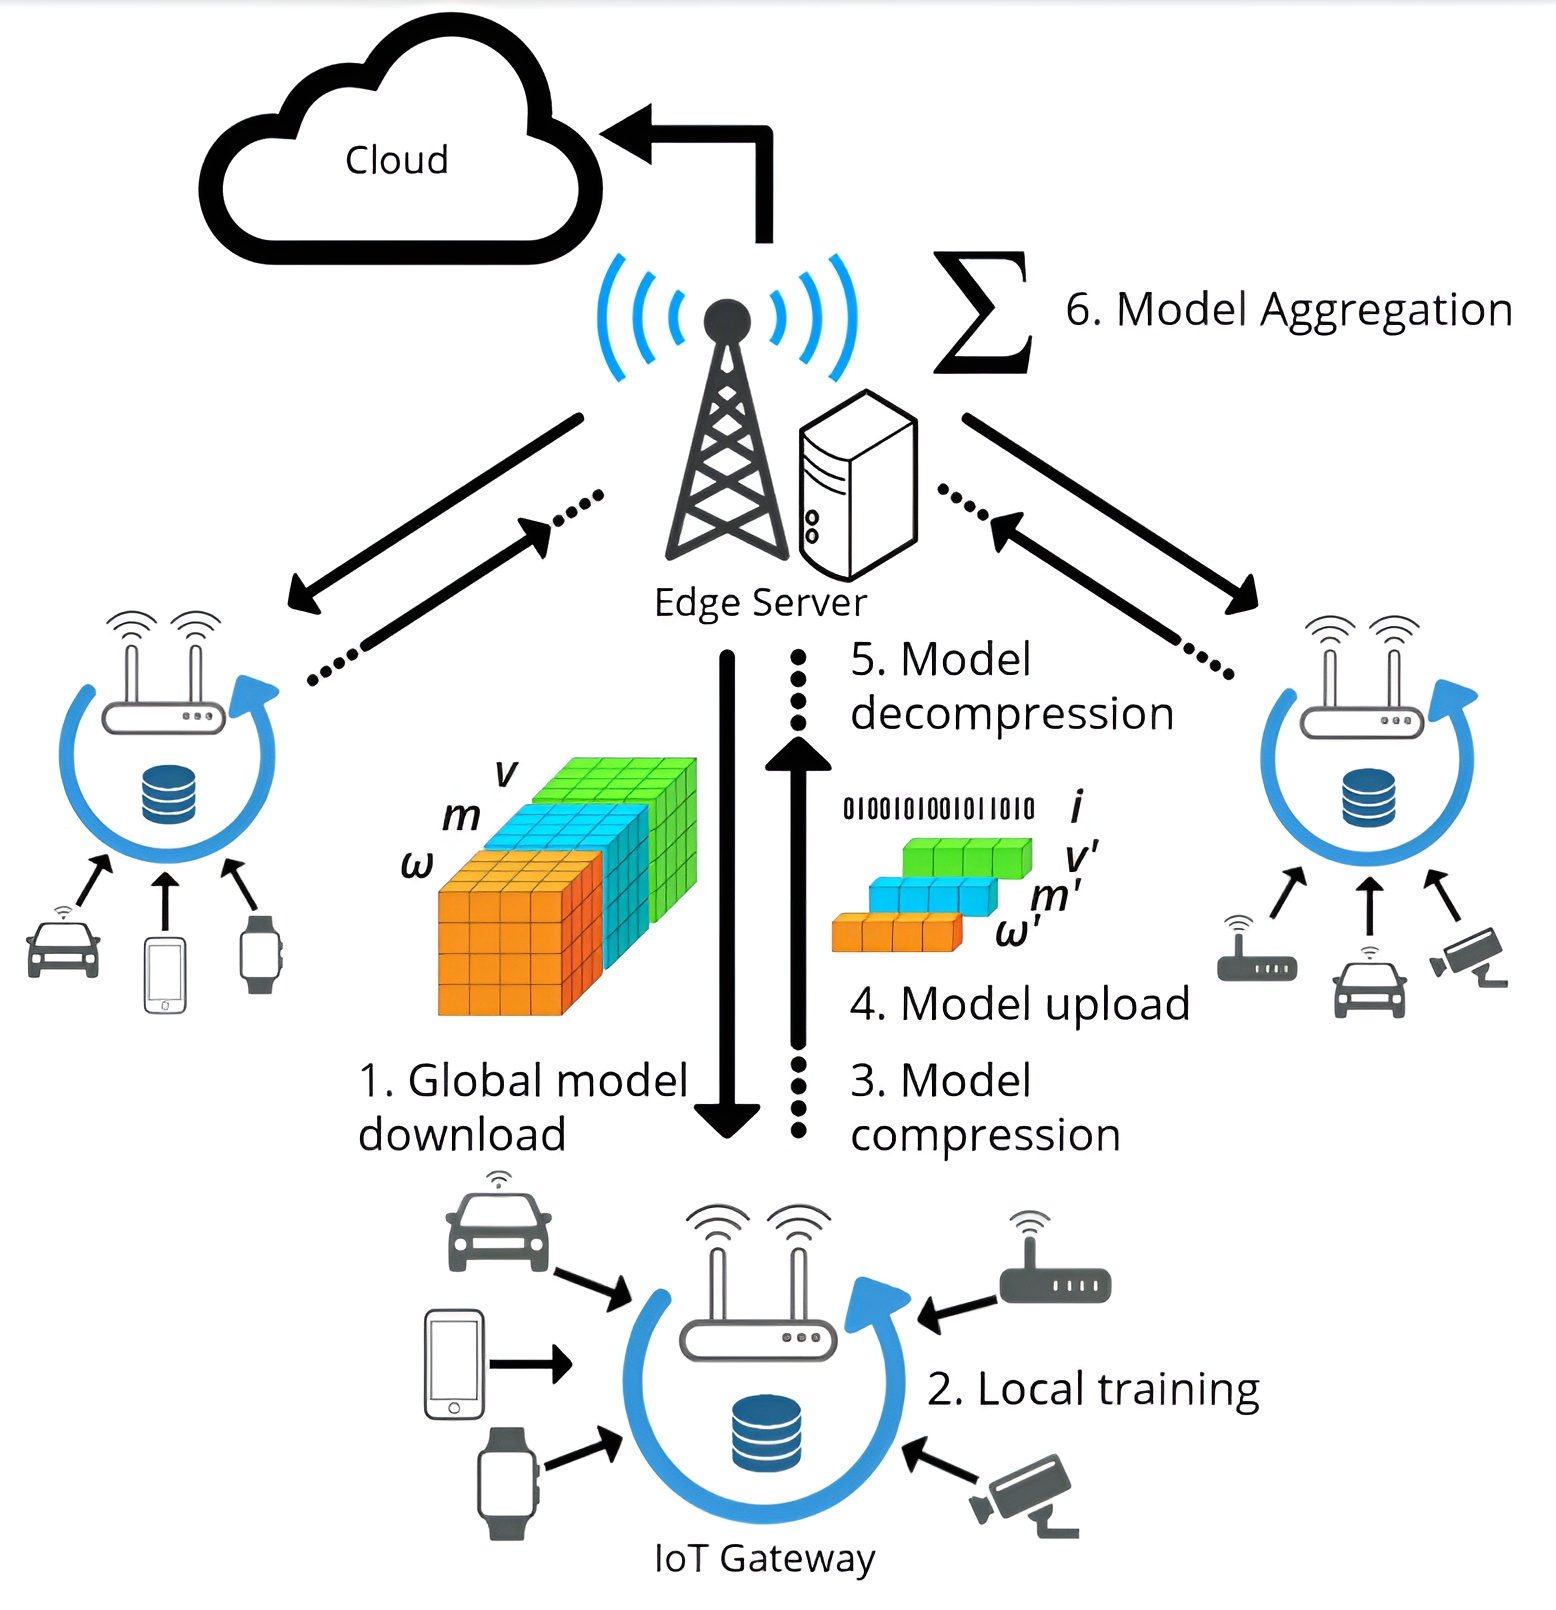
\includegraphics[width=0.5\textwidth]{archivos/img/teoria/fl.jpg}
    \caption{Esquema genérico de un sistema \gls{fl} \cite{mills2019communication}}
    \label{fig:fl}
\end{figure}


\subsubsection{Plano de datos inteligente}

\subsubsection{Infraestructuras flexibles y programables }




\subsection{Casos de uso verticales}



En resumen, el \gls{6g} promete llevar la conectividad y las comunicaciones inalámbricas a un nuevo nivel, superando las capacidades del \gls{5g} y habilitando una amplia gama de aplicaciones y servicios avanzados. Con velocidades ultra altas, latencia ultrabaja, conectividad ubicua y la integración de tecnologías emergentes, el \gls{6g} está destinado a impulsar la transformación digital en diversas industrias y habilitar un futuro aún más conectado e inteligente.

